\documentclass{beamer}
\usepackage[utf8x]{inputenc}
\usepackage[czech]{babel}
\usepackage{booktabs}
\usepackage{listings}

\usetheme[pageofpages=of,% String used between the current page and the
                         % total page count.
          bullet=circle,% Use circles instead of squares for bullets.
          titleline=true,% Show a line below the frame title.
	  titlepagelogo=opensuse,
          alternativetitlepage=true,% Use the fancy title page.
          ]{Torino}

\setbeamerfont{title}{series=\bfseries,size=\LARGE}
\author{Tom\'{a}\v{s} Chv\'{a}tal\newline {\small SUSE Packagers team}}
\title{Buildsystems and what the heck for we actually use the autotools}
\date{2013/07/19}

\AtBeginSection[]
{
	\setbeamercolor{background canvas}{bg=chameleongreen3}
	\begin{frame}[plain]
		\begin{center}\begin{huge}\textcolor{white}{\secname}\end{huge}\end{center}
	\end{frame}
	\setbeamercolor{background canvas}{bg=}
}

\AtBeginSubsection[]
{
	\setbeamercolor{background canvas}{bg=chameleongreen3}
	\begin{frame}[plain]
		\begin{center}\begin{huge}\textcolor{white}{\subsecname}\end{huge}\end{center}
	\end{frame}
	\setbeamercolor{background canvas}{bg=}
}

\begin{document}

\begin{frame}[t,plain]
\titlepage
\end{frame}

\section{Introduction}

\begin{frame}[t]{Who the hell is Tomáš Chvátal}
	\begin{itemize}
	\item SUSE Employee since 2011 - Team lead of packagers team
	\item Packager of Libreoffice and various other stuff for openSUSE
	\item openSUSE promoter and volunteer
	\item Gentoo developer since fall 2008
	\end{itemize}
\end{frame}

\section{Autotools process}

\begin{frame}{Complete autotools process}
	\begin{figure}
	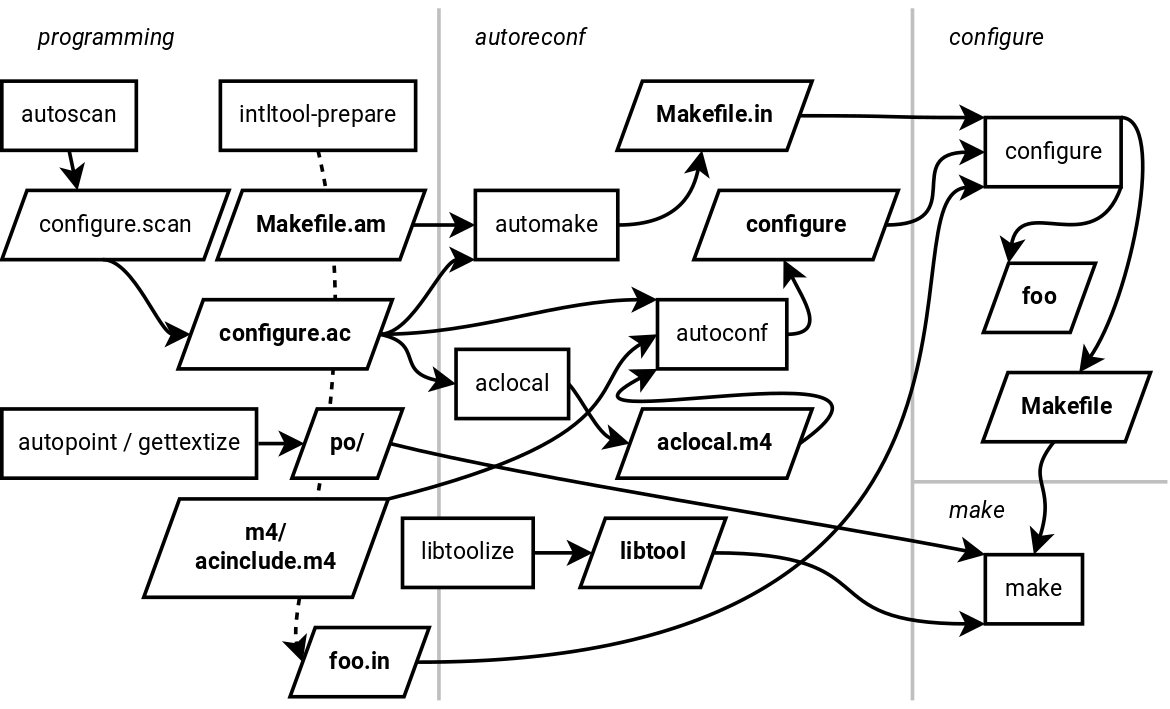
\includegraphics[width= 1.0\linewidth]{autotools.png}
	\end{figure}
\end{frame}

\section{Make}

\begin{frame}{Why not just a sh script?}
	\begin{center}
    \item Always recompiling everything is a waste of time and CPU power
	\end{center}
\end{frame}

\begin{frame}[t]{Plain makefile example}
	\begin{small}
	\lstinputlisting{makefile.txt}
	\end{small}
\end{frame}

\begin{frame}{Variables in Makefiles}
    \begin{itemize}
    \item Variables expanded using \$(), ie \$(VAR)
    \item Variables are assigned like in sh, ie VAR=value
    \item \$@ current target
    \item \$\textless the first dependent file
    \item \$\textasciicircum all dependent files
    \end{itemize}
\end{frame}

\begin{frame}{Well nice, but why autotools then}
    \begin{itemize}
    \item Makefiles can get complex fast (really unreadable)
    \item Lots of details to keep in mind when writing, small mistakes happen fast
    \item Does not make dependencies between targets really easier
    \item Automake gives you automatic tarball creation (make distcheck)
    \end{itemize}
\end{frame}

\section{Autotools}

\begin{frame}{Simplified autotools process}
	\begin{figure}
	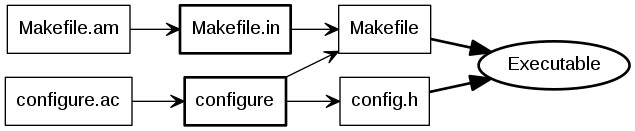
\includegraphics[width= 1.0\linewidth]{autotools_simple.png}
	\end{figure}
\end{frame}

\begin{frame}[t]{Autoconf/configure sample}
	\begin{small}
	\lstinputlisting{autotoolsconfigure.txt}
	\end{small}
\end{frame}

\begin{frame}{Autoconf syntax}
    \begin{itemize}
    \item The M4 syntax is quite weird on the first read
    \item It is not interpreted, it is text substitution machine
    \item Lots of quoting is needed, if in doubt add more []
    \item Everything that does or might contain whitespace or commas has to be quoted
    \item Custom autoconf M4 macros are almost unreadable
    \end{itemize}
\end{frame}

\begin{frame}[t]{Automake}
	\begin{small}
	\lstinputlisting{autotoolsmake.txt}
	\end{small}
\end{frame}

\begin{frame}{Basic rules}
    \begin{itemize}
    \item Always use just one Makefile.am in root folder
    \item All files that are to be distributed must be added to relevant parts or EXTRA\_DIST
    \item Always run make distcheck to verify your package really works
    \item Use check\_BINARIES/etc\ldots to have test phase
    \end{itemize}
\end{frame}

\begin{frame}{Variables for automake - SUFFIXES}
    \begin{itemize}
    \item \_PROGRAMS
    \item \_LIBRARIES DO\_NOT\_USE go for \_LTLIBRARIES
    \item \_SCRIPTS
    \item \_SOURCES
    \item \_HEADERS
    \item \_OBJECTS
    \item \_DATA
    \item \_LDADD
    \end{itemize}
\end{frame}

\begin{frame}{Variables for automake - PREFIXES}
    \begin{itemize}
    \item bin\_	will be installed to bindir
    \item sbin\_	will be installed to sbindir
    \item lib\_	will be installed to libdir
    \item noinst\_	will not be installed
    \item EXTRA\_	will be packaged upon make dist
    \item check\_	used only for make check
    \end{itemize}
\end{frame}

\subsection{Libtool}

\begin{frame}{Libtool versioning}
	\begin{itemize}
	\item Start with version information of ‘0:0:0’ for each libtool library
	\item If the library source code has changed at all since the last update, then increment revision (‘c:r:a’ becomes ‘c:r+1:a’)
	\item If any interfaces have been added, removed, or changed since the last update, increment current, and set revision to 0
	\item If any interfaces have been added since the last public release, then increment age
	\item If any interfaces have been removed or changed since the last public release, then set age to 0
	\end{itemize}
\end{frame}

\begin{frame}[t]{configure.ac changes}
	\begin{small}
	\lstinputlisting{autoconflibtool.txt}
	\end{small}
\end{frame}

\begin{frame}[t]{Makefile.am changes}
	\begin{small}
	\lstinputlisting{automakelibtool.txt}
	\end{small}
\end{frame}

\subsection{Autotools and windows}

\begin{frame}{Initial thoughts}
    \begin{itemize}
    \item Well for multiplatform support you can count on autotools on any UNIX-ish system
    \item On windows you have to use cygwin/mingw
    \item Per above you will spent bit of time getting that running
    \item You have to write yourself the .rc or rc.in file to be processed by cmake (see librevenge/etc.)
    \end{itemize}
\end{frame}

\begin{frame}[t]{Changes for configure.ac}
	\begin{tiny}
	\lstinputlisting{autoconfwindows.txt}
	\end{tiny}
\end{frame}

\begin{frame}[t]{Changes for Makefile.am}
	\begin{tiny}
	\lstinputlisting{automakewindows.txt}
	\end{tiny}
\end{frame}

\begin{frame}{Additional points for Makefile.am}
    \begin{itemize}
    \item Always pass -avoid-version to libtool
    \item Remember to add the resource file to \_DEPENDENCIES
    \item Script to compile the .lo files https://github.com/AbiWord/enchant/blob/master/lt-compile-resource
    \end{itemize}
\end{frame}

\begin{frame}{Autotools usability}
    \begin{itemize}
    \item Not hard as people are led to believe -> you can deploy it unless your files are too messy
    \item It, because of mingw, produces slower binaries than MSVC
    \item Most people are fine with it, but if not use Visual Studio project file and be done
    \item For .rc files you usualy have to use some shellscript as libtool has no clue
    \end{itemize}
\end{frame}

\section{CMake}

\begin{frame}{What are the benefits?}
	\begin{itemize}
    \item No libtool!
    \item Multiplatform generator for free Mac/Win/Linux...
    \item Can swap make for ninja
	\end{itemize}
\end{frame}

\begin{frame}{Any disadvantages?}
	\begin{itemize}
    \item FindBLA.cmake are sometimes pretty crappy
    \item If you rely on just .pc files you loose multiplatformity
    \item Can get unreadable fast
    \item Conflicting guides online, fine when you have someone to ask
    \item Distribution archive generator using CPack confuse many people
	\end{itemize}
\end{frame}

\begin{frame}[t]{CMake example}
	\begin{small}
	\lstinputlisting{cmakeexample.txt}
	\end{small}
\end{frame}

\begin{frame}[t]{CPack example}
	\begin{small}
	\lstinputlisting{cpackexample.txt}
	\end{small}
\end{frame}

\section{Reading}

\begin{frame}{Reading}
	\begin{figure}
	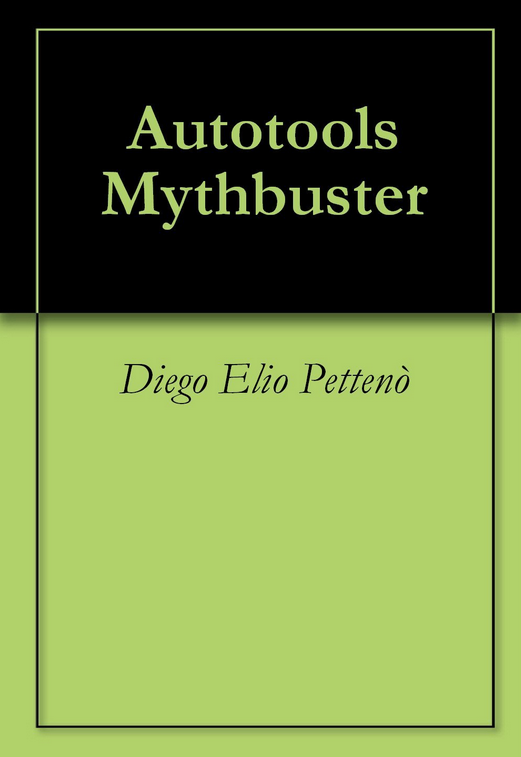
\includegraphics[width= 0.4\linewidth]{mythbuster.png}
	\end{figure}
\end{frame}

\section{Endnote}

\begin{frame}{Thanks}
	\begin{center}
	Thank you for your attention.
	\end{center}
\end{frame}

\end{document}

